\section{Knowledge Checklist}

Topics are divided up as best we can, to group things together logically.

Note that throughout, there is a general standing rule of ``you should know (abstract concept)'' also meaning ``you should be able to apply / recognise (abstract concept)'' if you're given a practical example!

\subsection{Fundamentals of Version Control}

You should understand the importance, potential advantages, and fundamental concepts of using version control for your (software) projects.

You should be familiar with fundamental \codeWord{git} functionality, workflow, and terminology.

\begin{itemize}
  \item What a repository is.
  \item The staging area, and the \codeWord{add} command.
  \item The repository history, what ``a commit'' is, the \codeWord{commit} command, and how to review history either graphically or via the \codeWord{log} command.
  \item Remotes, and the \codeWord{push}, \codeWord{pull}, and \codeWord{clone} commands.
  \item Branches, and the \codeWord{checkout} / \codeWord{switch}, \codeWord{branch} commands.
  \item Merges, the \codeWord{merge} command, and merge conflicts (how they arise, what they are, how they're resolved).
\end{itemize}

\subsection{Collaborative Software Projects}

You should understand the distinction between GitHub and Git.

You should be aware of important metadata files that should be provided as part of a software project being hosted on GitHub, and the reason for including them.
In particular:

\begin{itemize}
  \item The \codeWord{README} file, and its inclusion of the basic ``need-to-know'' introduction that a newcomer to the project requires.
        Or contains redirection to this information if it is hosted elsewhere.
  \item A \codeWord{LICENSE} file, to determine what can / cannot be done with the project.
  \item A \codeWord{CITATION} file, to ensure that appropriate credit is provided to the developers / maintainers, and the software can be easily referenced.
\end{itemize}

You should also be aware of the general folder structure of a software project on GitHub; being able to recognise the various files and folders that pertain to the tests, source code, documentation build, GitHub and Git configuration, etc.

You should understand what a fork of a GitHub repository is, and how to make contributions to open-source projects using them.
You should understand why external collaborators are expected to use forks, rather than direct access via clones, to contribute to projects.

You should have a clear understanding, and practice participating in, the development life cycle.
You should be able to justify why, and explain how, each step of the life cycle is conducted.

\begin{itemize}
  \item The use of issues for tracking work to be done, reporting bugs, or having discussions about new features.
  \item The use of branches for feature development.
  \item Use of pull-requests (PRs) for suggesting changes.
  \item Importance of code review prior to approval and PR merging.
  \item Any additional safeguards; such as testing, continuous integration workflows, or documentation checking.
\end{itemize}

You should understand that there are different approaches to development; in particular the Agile and Waterfall strategies.

\subsection{Python Knowledge}

You should have a firm grasp of the fundamentals of the Python language, including its syntax.

\begin{itemize}
  \item You should be able to write control-flow blocks, such as \codeWord{if}/\codeWord{elif}/\codeWord{else} blocks, \codeWord{for}-loops, and \codeWord{while}-loops.
  \item You should understand the fundamental Python data-types, and be comfortable working with container types like \codeWord{list}s, \codeWord{dict}s, and \codeWord{tuple}s.
  \item You should be able to write your own Python functions; and understand what is meant by an input argument, variable positional / variable keyword input arguments, and the return value.
  \item You should be able to understand Python class declaration and creation, and know the importance of the \codeWord{\_\_init\_\_} constructor method.
\end{itemize}

You should be aware that the Python standard library comes with functionality for reading JSON, CSV, (plain)text, and other common file types.
You should also be aware that there are additional Python libraries for handling and working with scientific data, like NumPy and Matplotlib.
Whilst you may be familiar with using some of these libraries (as you likely will use them during the class exercises or in the group assignment); you are not expected to be able to remember how to conduct complex workflows with them from memory, but should be able to make use of these libraries if given access to the documentation.

You should understand how to use the Pytest testing framework to write and run tests in Python.
You are not expected to remember how to setup shared fixtures or mocks from memory.
You are expected to be able to use the \codeWord{pytest.raises} context to check for errors being thrown.

You are expected to understand what a Python docstring is, how to write one, and to be able to extract information about a function / class from one.
You are not expected to remember any particular conventions for docstring layout, but you should be able to write docstrings whose style is consistent with those in an existing codebase.

You are expected to recognise the layout / structure of the source code for a Python package.
You should also recognise / understand what the purpose of the \codeWord{pyproject.toml} file is within such projects, though you are not expected to be able to create / write one from scratch yourselves.
You should still understand what information is placed inside this file.

You should be able to write command-line interfaces for certain package functions, given the reference material for a library such as ArgParse.

\begin{figure*}[h!]
  \centering
  
\includegraphics[scale=0.25]{images/simpsons-matplotlib.jpg}
  \caption{\label{fig:simpsons-interview} Matplotlib is one such powerful library that it would be unrealistic to expect you to be able to use in the exam without access to the documentation.}
\end{figure*}

\subsection{Working with Files}

You should be familiar with common (human-readable) data-file types, such as CSV, JSON, and YAML.
You should also have a high-level understanding of when someone may want to use one of these particular file formats over the others to store their data, and be able to apply this understanding to practical examples.
For example, CSVs excel at storing tabular data, but JSON and YAML are superior when the data is irregular or non-homogenous.

The distinction between plaintext data formats and binary data formats (like PDF, npz, ZIP, etc).

You should understand why we may want to prevent certain files or folders from being added to a (git) repository, and how this can be done with a \codeWord{.gitignore} file.
For example; preventing data files that do not form part of the software code / should not be publicly shared from being included in the repository history, or preventing a user's particular IDE settings from being committed to a repository.
You should be able to examine a \codeWord{.gitignore} file (or snippets thereof) and understand the rules being implemented by the file.

\subsection{Testing and Debugging}

You should understand the importance of providing (working!) tests for a codebase / software project, and keeping them up-to-date.

You should understand, be able to describe / define, and identify, the different types of tests that might be found in a codebase.
You should also be able to explain why (either abstractly or with context) each type of test might be used / found in a codebase:

\begin{itemize}
  \item Unit tests
  \item Negative (or failure-case) tests
  \item Mock tests
  \item Integration (or system) tests
\end{itemize}

You should understand what makes a good test; such as covering edge-cases, expected failures, and using simplified / controlled inputs and outputs to make verification easier.
You should be able to design tests based off these principles, given a particular codebase or function to work from.
You should also be able to recommend changes, additions (and possibly deletions) to test coverage / cases based on your understanding of the above.

You should be aware of the connections between a test suite and documentation, continuous integration, debugging, and PR review.
You should also be aware of how to exploit these connections to their full benefit.

You should be able use the bisection method, and \codeWord{git bisect}, to locate bugs within history.
This process may possibly be supported by an existing test suite.

You should know, understand, and be able to explain the principles of test-driven development.

\subsection{Documentation}

You should understand why it is important for all software projects to provide some form of documentation for both users and developers / maintainers.
You should also know (in the abstract) what information you expect to find / provide within project documentation.

You should be aware that there are existing tools for generating rich-format documentation (HTML / websites, etc) from plain-text files and source code.
(You will likely have already encountered Sphinx during the assignment, which is one such tool).
You should be able to explain why the generated documentation is not tracked by the repository it is stored in, as well as any additional integrations that a documentation build may have with concepts like continuous integration, developer practices, and PR review.

Understand the importance of documenting your code using in-line comments, expressive (self-reading / self-defining) code, and docstrings.

Given context, you should be able to write basic user / developer documentation, or simple examples for a codebase.
You should also be able to write docstrings in a particular format / style, given a codebase with existing examples or developer documentation that provides a clear style.

\subsection{Packaging and Libraries}

You should know what it means for a project to depend on, or be a dependency of, another library or package.

You should be able to assess both the benefits and potential drawbacks of having a project depend on an external (or 3rd-party) library.
You should also know what to look for in an external library to help you make this decision; such as the quality of their tests and documentation, how well-maintained or frequently updated it is, whether it provides too little / too much functionality outside of what you need, etc.

You should understand the difference between a collection of scripts and a package / library.
You should be able to write scripts that use functionality from a library / package that you have written or been provided.

\subsection{Code Structure and Design}

You should be able to recognise abstract design patterns in particular codebases, and be able to write code to adhere to a particular design pattern.
You are not expected to memorise specific design patterns, but should be able to identify whether a design pattern is being used (or not) given its description.

You should know what the term ``refactoring'' or ``to refactor'' means in the context of a software project.
You should be able to explain why refactoring can be useful, and identify candidates for refactoring / undertake this yourself if given a particular codebase.
You should also be aware of any features that should already be in place before undertaking refactoring (for example, tests!).

\begin{figure*}
  \centering
  
\includegraphics[scale=0.25]{images/beaver-refactorings.jpg}
  \caption{\label{fig:beaver-refactoring} Refactoring offers many advantages, but can be a major time-sink if the codebase has already grown quite large without any design structure being imposed at the beginning.}
\end{figure*}

\subsection{Profiling and Benchmarking}

You should be aware of the distinction between profiling and benchmarking code.

Profiling is timing the execution of a particular block of code; with the interest being in exploring how long the program spends on each particular line of code or within specific sub-functions, and how frequently these parts of the codebase are reached by the program.
Profiling is typically used to identify ``bottlenecks'' within the codebase, or to get an overview of the relative importance of improving the efficiency of one function over another.
For example; profiling may identify that a function \codeWord{f} is called 1000 times by some code, and takes 1 second to execute each time.
Whereas another function \codeWord{g} might be called only once, but take 10 seconds to execute.
In such a case, our conclusion from the profiling run might then be that we should actually focus on making a small 0.1 second improvement to \codeWord{f}'s runtime, as opposed to a 3 second improvement to \codeWord{g}'s, and should base our future design decisions on what helps \codeWord{f} run faster, rather than \codeWord{g}.

Benchmarking is timing the execution of a particular block of code, with the interest being in exploring how long the program takes to execute, as the inputs are varied / scaled.
Benchmarking is typically used to demonstrate how well a program scales onto larger data / input sizes, or provide results for comparison against projects that offer similar functionality (but perhaps in alternative programming languages).
Benchmarking can also flag when our code is performing - as a whole - above or below a certain expectation, and at which kinds of inputs that we see these deviations from theory / expectation.

You should understand \href{https://en.wikipedia.org/wiki/Big_O_notation}{``big-O'' notation} ($O(N^3)$, $O(a^N)$ etc) and its applications to benchmarking.
You should understand what it means for a quantity (say $t$) to scale exponentially or as a power-law, with another quantity (say $N$).
In each case, you should be able to infer a scaling relationship, and potentially estimate the various quantities that define the relationship, from plots or numerical information.

\begin{itemize}
  \item Power-law: $t$ scales $O(N^\alpha)$, so we expect that $t = \beta N^{\alpha}$ for some constants $\alpha, \beta$.
        The term ``polynomial growth'' or ``grows polynomially'' is sometimes used for the case where $\alpha > 0$.

        This scaling relationship looks (visually) linear on a plot of $t$ (y-axis) against $N$ (x-axis) with \textbf{log-log axes}.
        Equivalently, we could write
        \begin{align*}
          \log t & = \alpha \log N + \log\beta
        \end{align*}
        and check if we observe a linear trend when plotting $\log t$ (y-axis) against $\log N$ (x-axis) on normal axes.
        \begin{figure*}[h!]
          \centering
          \includesvg[scale=0.45]{images/power-law-scaling.svg}
          \caption{
            \label{fig:power-law-quantity-estimation}
            Estimating the constants $\alpha ( = 1.5)$ and $\beta ( = 3)$ from a benchmarking plot (of $t = 3N^{1.5}$).
          }
        \end{figure*}
  \item Exponential: $t$ scales $O(\alpha^N)$, so we expect that $t = \beta \alpha^{N}$ for some constants $\alpha, \beta$.
        This scaling relationship looks linear on a plot of $\log t$ (y-axis) against $N$ (x-axis) when using log-log axes.
        The gradient of said linear line is an estimation for $\log \alpha$, and the y-axis intercept an estimation for $\log \beta$.
        \begin{figure*}[h!]
          \centering
          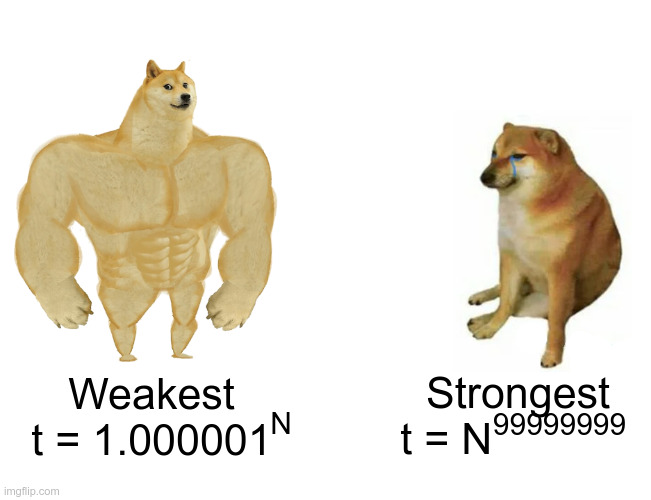
\includegraphics[scale=0.25]{images/doge-exp-vs-power.jpg}
          \caption{\label{fig:doge-scaling} Exponential growth is always faster than polynomial growth, even if polynomial growth starts off strong.}
        \end{figure*}
\end{itemize}
